\documentclass{book}
\usepackage{multicol}
\usepackage{graphicx}
\usepackage{multicol}
\usepackage{geometry}
\usepackage{array}
\usepackage{float}


\title{Gechman, Marvin - Project management of large software-intensive systems _ controlling the software development process-CRC Press (2019)}
\author{Abouhamze Fahime}
		
\begin{document}
	


\begin{multicols}{2}

basic “systems theory” that views the world as a complex system of interconnected parts, scopes the system by defining
its boundaries, and then makes simplified representations
(or models) of the system structure in order to understand
it and to predict the behavior of the system. At the highest
level, the essence of Systems Engineering is structure. System
Engineers understand the system by bringing structure to it
and by defining the set of elements, or parts, so connected or
related as to form the whole system.

Software Engineering can be considered a part of Systems
Engineering. On many programs and projects, Software
Engineering is located organizationally within the Systems
Engineering group. That is because the two disciplines are
not merely related, they are intimately interlaced. The important collaboration between system and Software Engineering
is discussed below and in Chapter 12. Whereas System
Engineers may manage the building of a dam or a bridge,
the creation of new models of automobiles, the launching
of satellites into space, or the development of new types of
electronic devices, Software Engineers deal with the software
aspects of those systems. Those aspects are never trivial.

It is important to understand what Systems Engineering
is not in the context of this Guidebook. Information
Technology (IT) departments in many organizations have
an important function called “Systems Engineering.” That
function typically deals with the operation and performance
of all the computers, corporate servers, networking, multicomputer systems, operating systems and other IT related
issues. That function is not the Systems Engineering function referred to in this Guidebook. I view each project as
one system, so I refer to the engineers working on a system as
“System Engineers.” “Systems Engineering” (plural) is used
only because that is what everyone calls it.

\textbf{1.4.3 The Collaboration of Systems and Software Engineering}

Software Engineering (SwE) and Systems Engineering
are tightly coupled in today’s software-intensive systems—and that includes essentially all major systems.

In nearly all application areas, including aerospace, education, medicine, transportation, etc., software-intensive systems are providing unprecedented system functionality. The
growth of software involvement is essentially exponential.
Using jet fighter airplanes as an example: The F16 in 1976
relied on software for about 40% of its capability; the F-22s
in 1997, relied on software for about 80% of its capability;
and in 2006 the F-35 relies on software for 90% or more of
its capability. The same growth of software for automobiles
has occurred as current vehicles have millions of lines of code
and the pinnacle is driverless cars, currently being tested,
that are controlled entirely by software.


Software considerations need to be involved in every system decision, and SwE expertise should be utilized throughout the Development Life Cycle by System Engineers. At the
same time, Software Engineers need to be continually looking at the impact their decisions make on the system, and they
must convey this information to the System Engineers. The
criticality of this collaboration and the exchange of information grows exponentially with the size of the program.

To ensure success, system and software requirements,
architectural design, implementation, integration and testing must be a collaborative effort between the two disciplines
and have the ability to evolve with changing customer or
environmental needs. The “Systems Engineering Acquisition
Team,” or the customer’s Program Office, is usually responsible for ensuring such participation exists. The Chief Software
Engineer, and relevant Software Engineers, should be members of the Systems Engineering Acquisition Team.

Early involvement of Software Engineering in the System
Life Cycle is a major help in mitigating the risks of excessive cost, effort and rework because poor system architecture choices can negatively impact the software development
effort. Chapter 12 is devoted to the detailed identification
and description of the collaborative tasks performed by
System and Software Engineering. In Chapter 12 that collaboration is discussed from two perspectives:

\begin{itemize}
	\item There are system development activities that are the
	responsibility of Systems Engineering, but these activities are supported by Software Engineering.
	\item There are software development activities that are the
	responsibility of Software Engineering, but these activities are supported by Systems Engineering.
\end{itemize}

\textbf{1.4.4 System Life Cycle Overview}
The System Life Cycle is a cradle to grave perspective starting
with an initial conceptual analysis of the proposed system
and ending with an ultimate replacement or retirement of
the system. The SLC is sometimes referred to as the “System
Acquisition Life Cycle.” Figure 1.2 should be carefully
reviewed as it is an important conceptual overview involving
the hierarchical relationship of:
\begin{itemize}
\item The System Life Cycle that includes System Definition,
Software Development Life Cycle and the System
Sustainment activities
\item The Software Development Life Cycle which incorporates part of System Definition, plus the Software
Implementation Process and the System Integration,Testing and Verification (System IT V)
\end{itemize}
(NOTE: Software Engineering literature sometimes
defines the acronym “SDLC” as the System Development 
Life Cycle; this Guidebook identifies the system-level life
cycle as the SLC.)

Although Figure 1.2 is an important overview, it is
intended to be a conceptual introduction to the architecture of the SLC process showing the five activities embedded within the SLC. Figure 1.2 will be expanded during
the discussion of life cycle processes in Chapter 3, with
additional figures that are elaborations of Figure 1.2.
Hardware development is performed at the same time as
the SDLC.

An easy way to understand the System Life Cycle can be
depicted using the well-known engineering V-chart modified to show the software development and typical review
process. As shown in Figure 1.3, the left side of the “V” contains the design activities and related reviews, and the right
side contains the integration and test activities and related
reviews.

Figure 1.3 does not contain all of the activities and
reviews; the complete process will be discussed in later 

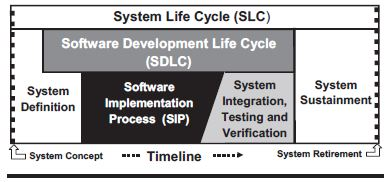
\includegraphics{Figure1.2}
Figure 1.2 Conceptual overview of the System Life Cycle

chapters and in Figures
3.3, 3.4, 4.4 and 12.2. Specific activities performed by Software Project Managers are covered in
subsequent chapters of this Guidebook, especially Chapter
2 which is entirely focused on SPM activities. Additional
system-related subjects discussed are:

\begin{itemize}
\item Systems Engineering activities are addressed in Chapter 10.
\item Software Engineering activities and the software development process are discussed in depth in Chapter 11.
\item Chapter 12 describes the collaborative activities of
systems and Software Engineering along with more
details of the system and software life cycles.
\item Integration, Testing and Verification activities are covered in several sections.
\item The System Life Cycle does not end at the release of
a software product into production. A working product in the hands of the customer is just the beginning
of the longest and most costly portion of the System
Life Cycle—System Sustainment, often referred to as
“System Maintenance,” is covered in Chapter 16.
\end{itemize}

\textbf{1.4.5 System Boundaries}
You must provide the context for your project by defining the
boundaries and scope of your contractual responsibilities. In
other words, what your project includes and what it does not
include. In addition to the starting and ending points, you
need to know the origin of the inputs as well as the specific
destination of the outputs of your interfaces.

Boundaries are important because most systems interact


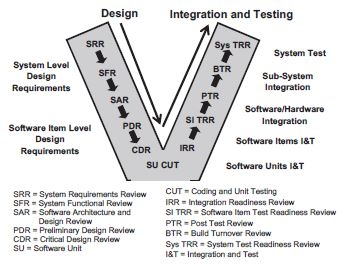
\includegraphics{Figure1.3}
 Figure 1.3 System Development Life Cycle V-chart.

with other systems. These interdependencies between systems  
can be complex and can take an inordinate amount of your
resources. Even if they are not your responsibility, to make
everything work together seamlessly, you and your team
must define and describe these boundary interfaces because
they can have a huge impact on your cost and schedule.

\textbf{1.4.6 System of Systems}
The software-intensive system you are developing can incorporate one or many systems within the boundaries of your
project. Your project could then be considered a System of
Systems (SoS). An SoS can become incredibly complex as
illustrated by the Commercial Aircraft SoS in Figure 1.4.

A System of Systems can be viewed as a set, or arrangement of systems, that results when independent and useful systems are integrated into a larger system that delivers
unique capabilities. A subsystem is a set of elements, which
may be a system itself, but also is a component of a larger system. Subsystems are sometimes called segments.

During system development, integration and operational
problems frequently arise due to inconsistencies, ambiguities, and omissions in addressing quality attributes between
system and software architectures. These problems are
compounded in a SoS. The architecture framework for the
Department of Defense is called DoDAF. It provides a good
set of architectural views for a SoS architecture. It is important to remember that identifying and addressing quality
attributes early in the process, and evaluating the architecture to identify risks, is a key to success.

In addition, end-to-end mission threads, augmented with
quality attribute considerations, are needed to help develop
and later evaluate the SoS and the constituent system and
software architectures. If you are the Project Manager of an
SoS, you must track it carefully.

Each of the Commercial Aircraft systems identified in
example Figure 1.4 are themselves considered a SoS as they
can be further broken down into component systems as 

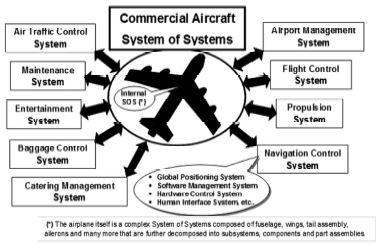
\includegraphics{Figure1.4}
Figure 1.4 Context of a System of Systems.

shown for the Navigation Control System. The elements of
a SoS must be broken down into manageable components.
If your project is part of a System of Systems, the need to
clearly define the scope and boundaries of each system element
becomes even more critical.


\textbf{1.4.7 The One-Page Big Picture Flowchart Overview}


The following lesson learned is one example, of many in my
career, where a one-page big picture flowchart overview was
a key mechanism for understanding and identifying required
system functionality with the help and concurrence of the
customer.

\textbf{Lessons Learned}. Early in my career, I was
working for a Washington, DC, think tank,
and we had a contract to automate the processes
of the Small Business Administration (SBA).
I was the Lead Software System Engineer. The
SBA had previously hired two different software
contractors, but nothing usable was produced.
I asked them to show me what had been done
and was taken to what was essentially a large
closet filled with boxes of punched cards (yes it
was a long time ago). Each of the two previous
contractors had different sets of punched cards
with different formats. So I then asked to see
the documentation that went with the punched
cards and the expected response was: we don’t
have any documentation.

I realized the previous work had been performed by hackers who either had no idea what
they were doing, or they were trying to automate
small tasks. I had to start from scratch. I asked
the SBA to set up an appointment for me to talk
in depth with someone who has a good understanding of the overall SBA process.

Being somewhat naïve at that time, I was
surprised to learn that there was no such person! There were people who knew exactly
what processes were being followed at the SBA
Headquarters operation in Washington, DC,
but in order to understand the process at a district office, I would have to visit one of them. I
obtained all the information about the processes
at the SBA Headquarters and then traveled to
one of the largest SBA district centers in Dallas.

After returning from Dallas with ample
information, I prepared an implementation plan
and report. Although I had a lot of data, I was
able to identify the salient operations of the over all SBA process and converted it into a flow chart




where the entire SBA process was depicted on one
page (a large 24 by 30 inch sheet that folded up
nicely into a pouch in the back of the report). It
was the first time SBA management had a big picture understanding of the overall SBA process—
and on one page!

That one-page flow chart was instrumental
in determining “what” to automate and it was
also invaluable in obtaining understanding and
approval by the customer. To keep it simple, the
flowchart contained only the top-level processing
tasks making it much easier to understand what
needed to be automated and much easier to discuss the automation tasks with SBA management.

There are two reasons for telling this story:
\begin{itemize}
\item The advantages of a one-page flowchart overview when
discussing the project with the customer—especially
top management.
\item Why the “big picture” view is important for every
system and invaluable for large or complex systems.
Keeping it as simple as practical was a critical element
of success for this system as well as every other system
I worked on.
\end{itemize}

For complex implementations, all the functionality cannot
be put on one page. However, a very top-level overview of the
process can be on one page, followed by one-page expansions
of each box shown on the top-level flowchart. You can continue
that process until you peel down to the precise details needed
to describe the overall design for subsequent implementation
by the Programmers.

Understanding the big picture is crucial.

\textbf{Lessons Learned.} Sometimes having a one-page
big picture overview can get you in trouble. For
example, I once went to work for a computer firm
developing sophisticated solutions to data storage
and retrieval systems. They had this one fellow
who was brilliant and productive, so they let him
get away with a lot. His approach was to make
his system designs complex and confusing, and
his briefings and documentation were the same,
so no one really understood exactly what he was
doing. I reviewed his report, combined the similar tasks, eliminated the side issues, and simplified it the point where I could graphically show
essentially what he was doing on one page. When
I presented this chart at the next update—well,
let’s say if he had a gun I would have been shot.
He barely spoke to me again, but now everyone
knew what he was doing.

\textbf{1.5 Software Project Planning}

\textit{Planning is critical; if you don’t know where you
are going—you will never get there!}

Although software planning is performed throughout
the software life cycle, strategic planning up front usually
makes the difference between success and failure of a software
development project. This Section describes the two fundamental pillars of software project planning, the Software
Development Plan and the Work Breakdown Structure, plus
the potential need for a Project Charter.

\textbf{Project Charter.} Preceding the formal planning process,
an optional Project Charter may have to be produced. The
Project Charter should be developed by the customer or organization requesting and funding the project prior to the formation of a Project Team. The Project Charter is a very high-level
document, and it serves as the starting point for the SDP. It
describes why the project has been initiated, what the project will accomplish, generally how and when the product will
be developed or provided, who is responsible to perform the
work, and who benefits from the project products or services.

Contents of the Project Charter, sometimes called the
Project Vision or Scope Plan, is obviously dependent on the
characteristics of the project. However, the following is a
general outline of its contents:

\begin{itemize}
\item Title of the Project: Descriptive but not too lengthy.
\item Purpose of the Project: Overall scope of the project
including a brief statement of the problem(s) the project will solve, but not the solution.
\item Expected Results: Description of what will be accomplished and when the project is planned to be completed. Results must be measurable qualitatively or
quantitatively.
\item Assumptions: Includes the conditions, environment or
ground rules that will govern the execution of the project, and which must be acknowledged for its successful
completion.
\item Roles and Responsibilities: Identifies key project participants, their roles and responsibilities, including the
Project Manager and major supporting agencies.
\item Authority Statement: The level of authority and approval
given to the Project Manager.
\item Signatures: Signoffs of key project stakeholders
acknowledging their concurrence.

\end{itemize}

\textbf{1.5.1 Software Development Plan}
\textit{
A poorly planned software development effort
is likely to fail—that makes the SDP a critically
important software management tool for essentially
all software development efforts.}



Every software development program should have a
Software Development Plan, but for large programs it is a critical element for success. The SDP may also be called a Project
Plan, Project Work Plan, Software Project Management Plan,
Software Development Management Plan or something similar,
but it is called an SDP in this Guidebook. \textit{The SDP documents
the processes by which the software will be designed, developed,
integrated, tested and managed.}

An SDP, or similar document, is required by essentially
all software development standards. It is prepared by the
software organization performing the development. For government work, it is typically required and submitted with
the developer’s (contractor’s) proposal. Whenever the SDP is
referred to in this Guidebook, replace it with the equivalent
document name used by your program or organization.

The SDP is focused on what will be done and should be
backed up with detailed operational procedures that describe
how to do it. It is not uncommon for the detailed standards
of corporate operational procedures to fill a bookshelf. But
even for large systems, the SDP itself is seldom larger than
200 pages. However, the SDP package may include annexes or
addenda that could be bound with the SDP or bound separately. SDP packages on large programs can become quite
large and may include annexes containing plans for management and control of quality, risks, configuration, metrics,
testing, subcontractors, budgets, reviews, resources, reuse,
integration and test, roles and responsibilities, etc.

The SDP describes the set of processes, methodologies,
tools, development and testing environments, and life cycle
models, appropriate for the scope and complexity of your
project, that will be used consistently by all team members.
Teammates and subcontractors may need to prepare sitespecific versions of the project-level SDP to address issues of
concern only to them, as long as their site-specific SDP does
not conflict with the project-level SDP. Specific conflicts
with the project-level SDP is acceptable as long as formal
waivers are requested and approved. The SDP is discussed in
more detail in Subsection 5.1.1, and Appendix F contains an
example annotated outline of the SDP.

\textit{An incomplete, poorly written, unorganized or
inadequate SDP is a clear red flag!}

\textbf{Lessons Learned.} Do not underestimate the
importance of the SDP. Bidders on government
contracts with a deficient SDP are significantly
decreasing their chances of winning contracts,
and those with a deficient SDP who are awarded
contracts have an historically high probability of
cost and schedule overruns. A good SDP will significantly increase the probability of a successful
software-intensive system. I was on Government
Contract Source Selection Teams and could not 


believe the quality of SDPs ranging from poor to
excellent submitted by major aerospace corporations. Spend the time up front to produce a good
SDP because it will have a big payoff in terms
of winning contracts and especially during management of the project.

\textbf{1.5.2 Work Breakdown Structure}
The Work Breakdown Structure is a key software budgetary planning and control activity. The WBS organizes and
decomposes, in a hierarchical structure, all the project tasks
into smaller, more manageable and controllable components. It is product-based and includes the development of
all hardware, software and documentation products plus
requirements analysis, testing and anything else that must
be accomplished to finish the project and deliver the system.
The WBS provides a strategy for completing the project by
dividing the entire project into a hierarchical logical breakdown. Graphically, the WBS is normally shown as a tree
structure, as depicted in the example in Figure 1.5.

The WBS tree structure should be augmented with documentation in the form of an annotated outline that contains
more details than shown in a figure similar to Figure 1.5. On
smaller projects, it is not absolutely necessary to have both
the tree structure and the outline. In its simplest form for
small projects, the WBS can be portrayed with yellow sticky
notes organized on a whiteboard.

The number of levels in a WBS must break down the
planned work into manageable tasks and, as a general ruleof-thumb, they should not be larger than what can be accomplished in a short time period (varies by project but about
2–3 weeks). The WBS is also extremely useful in preparing
network diagrams as described in Section 8.4. Updating the
WBS, as required, should be performed by following the
change control process described in Section 6.4.

There are many benefits you can realize from the WBS
including:

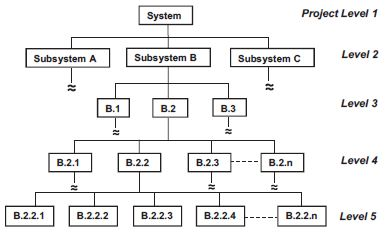
\includegraphics{Figure1.5}
Figure 1.5 Example of a tree-structured WBS.
 
 
\end{multicols}
\end{document}		
		
	    
		
		